\documentclass[aspectratio=169]{beamer}
\usetheme{Madrid}
\usepackage{booktabs}
\usepackage{graphicx}
\usepackage{array}

\title{Branch Specialization Checkpoint}
\subtitle{All-Layout Local-Weight Sweep}
\author{Branch Specialization Project}
\date{2026-05-22}

\begin{document}

\begin{frame}
  \titlepage
  \vspace{-0.5em}
  \begin{center}
    Checkpoint reason: full 100-model grid refines the capacity-attractor mechanism.
  \end{center}
\end{frame}

\begin{frame}{Question}
  \textbf{Project question:} Does structural heterogeneity lead to stable functional specialization?

  \vspace{0.8em}
  Previous result: for one layout, reducing local-task pressure let induction use
  the 64-dim head.

  \vspace{0.8em}
  This checkpoint asks whether that result generalizes across all four 64-dim
  placements:
  \begin{itemize}
    \item [64, 16, 16, 32]
    \item [16, 64, 16, 32]
    \item [16, 32, 64, 16]
    \item [16, 16, 32, 64]
  \end{itemize}
\end{frame}

\begin{frame}{Setup}
  \begin{itemize}
    \item Task has two roles: local copy and induction-style continuation.
    \item Local weight swept: 0.00, 0.01, 0.10, 0.25, 1.00.
    \item Induction weight fixed at 1.00.
    \item Four heterogeneous layouts, five seeds each: 100 models total.
    \item Role score: single-head causal ablation loss delta.
    \item Main readout: whether the role's top causal head is 64-dim.
  \end{itemize}
\end{frame}

\begin{frame}{Aggregate Evidence}
  \begin{center}
  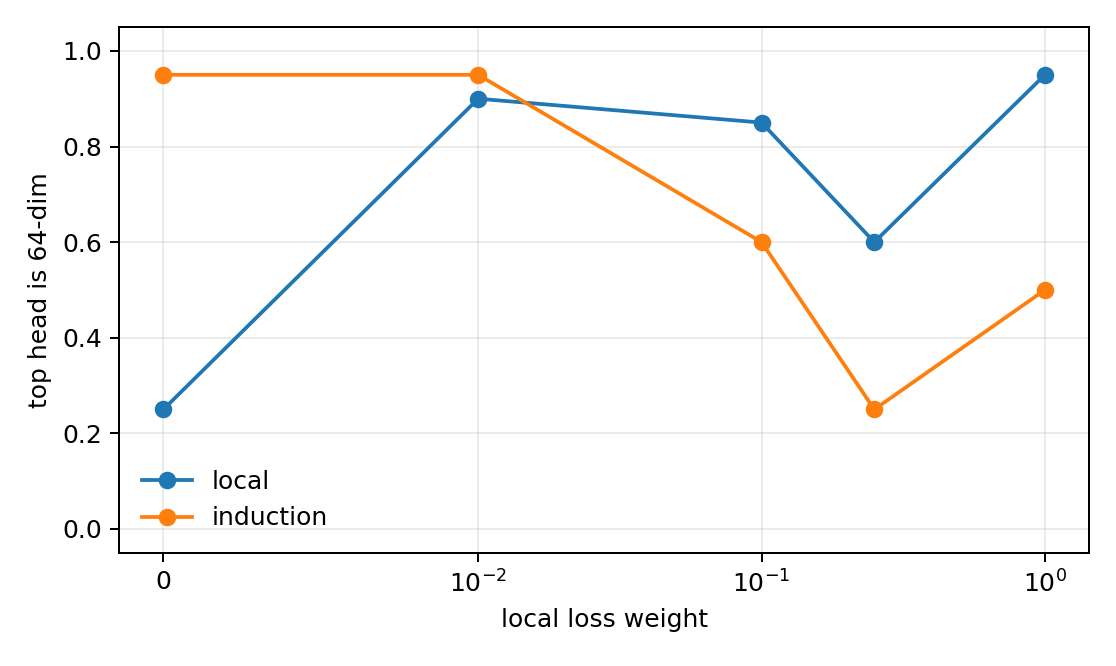
\includegraphics[width=0.82\linewidth]{figures/aggregate_top64_by_weight.png}
  \end{center}

  \vspace{-0.4em}
  \small
  Low local pressure leaves induction on 64-dim heads. Moderate local pressure
  often displaces induction to secondary heads.
\end{frame}

\begin{frame}{Aggregate Table}
  \begin{center}
  \scriptsize
  \begin{tabular}{rrrrrr}
    \toprule
    Local weight & Models & Local acc. & Induction acc. & Local top 64 & Induction top 64 \\
    \midrule
    0.00 & 20 & 0.2006 & 0.9979 & 0.25 & 0.95 \\
    0.01 & 20 & 0.9955 & 0.9979 & 0.90 & 0.95 \\
    0.10 & 20 & 0.9998 & 0.9983 & 0.85 & 0.60 \\
    0.25 & 20 & 1.0000 & 0.9986 & 0.60 & 0.25 \\
    1.00 & 20 & 1.0000 & 0.9993 & 0.95 & 0.50 \\
    \bottomrule
  \end{tabular}
  \end{center}

  \vspace{0.6em}
  Induction top-64 rate changes from 19/20 at low local pressure to 5/20 at
  local weight 0.25.
\end{frame}

\begin{frame}{Layout-Specific Evidence}
  \begin{center}
  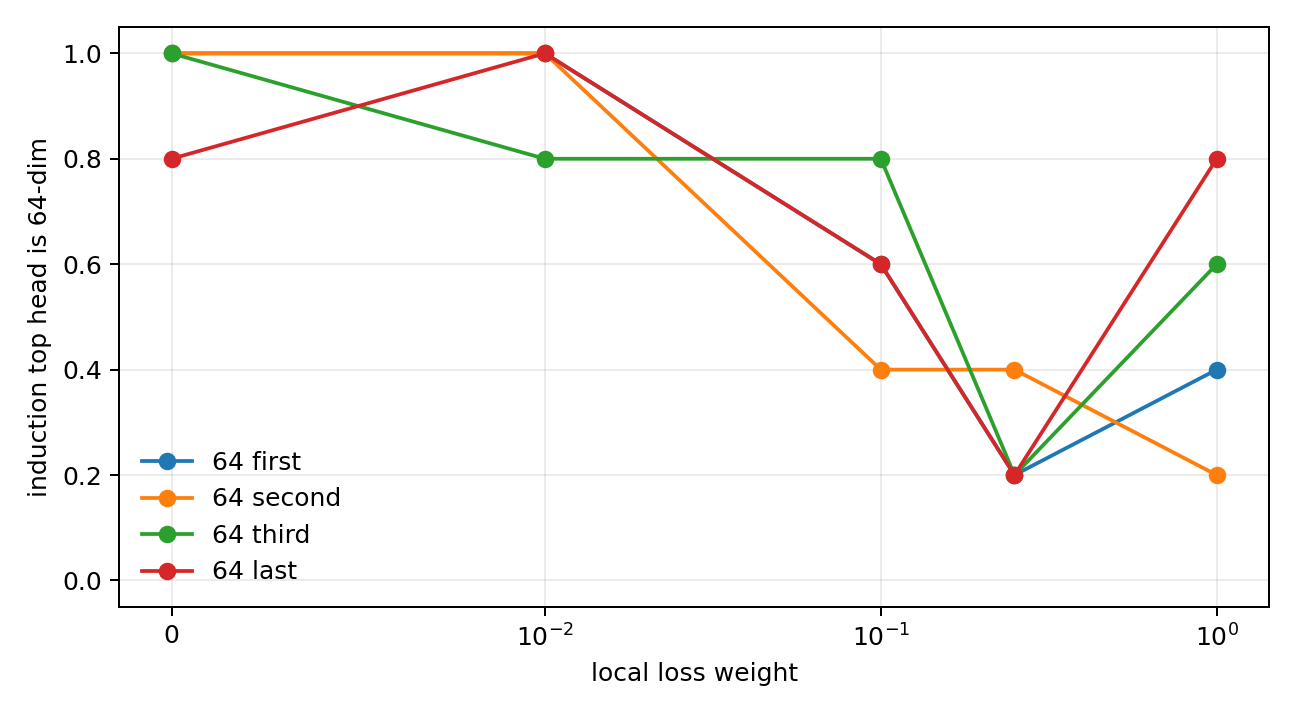
\includegraphics[width=0.82\linewidth]{figures/induction_top64_by_layout_and_weight.png}
  \end{center}

  \vspace{-0.3em}
  \small
  The pressure effect generalizes, but the curve is not strictly monotonic and
  remains layout-sensitive.
\end{frame}

\begin{frame}{Interpretation}
  \textbf{Supported:}
  \begin{itemize}
    \item The 64-dim head is a real attractor for induction when local pressure is absent or tiny.
    \item Local pressure changes role allocation among structural slots.
    \item Heterogeneity stabilizes slot formation across seeds.
  \end{itemize}

  \vspace{0.5em}
  \textbf{Not supported:}
  \begin{itemize}
    \item A fixed semantic taxonomy where large heads always mean induction/global.
    \item A one-variable monotonic law from local weight to induction displacement.
  \end{itemize}
\end{frame}

\begin{frame}{Updated Mechanism}
  Best current mechanism:

  \vspace{0.8em}
  \begin{quote}
    Structural heterogeneity creates capacity-attractor slots; role allocation
    among those slots is pressure-sensitive, layout-sensitive, and
    optimization-basin-sensitive.
  \end{quote}

  \vspace{0.8em}
  This supports functional specialization stability in the toy setting. It does
  not yet establish functional modularity.
\end{frame}

\begin{frame}{Decision}
  Continue Phase 3, but with the narrowed claim.

  \vspace{0.8em}
  Next decisive experiment:
  \begin{itemize}
    \item Add two-attractor layouts, e.g. [16, 48, 48, 16], [48, 16, 48, 16], [48, 48, 16, 16].
    \item Test whether local and induction split more cleanly when there are two medium-large heads.
    \item If displacement weakens, it directly supports the capacity-attractor competition mechanism.
  \end{itemize}
\end{frame}

\begin{frame}{Sources and Provenance}
  \scriptsize
  \begin{itemize}
    \item Report: \texttt{doc/phase3\_toy\_competition\_all\_layout\_weight\_sweep.md}
    \item Training script: \texttt{scripts/toy\_competition\_head\_dim\_intervention.py}
    \item Analysis script: \texttt{scripts/analyze\_competition\_all\_layout\_weight\_sweep.py}
    \item Combined analysis: \texttt{results/phase3\_toy\_competition\_all\_layout\_weight\_sweep/}
    \item Deck data snapshot: \texttt{presentations/2026-05-22-1135-all-layout-weight-sweep/data/}
  \end{itemize}
\end{frame}

\end{document}
